\documentclass{article}

\usepackage[english]{babel}
\usepackage[utf8]{inputenc}
\usepackage{amsmath}
\usepackage{graphicx}
\usepackage[colorinlistoftodos]{todonotes}
\usepackage{amsfonts}
\usepackage{titling}
\usepackage{indentfirst}
\usepackage{adjustbox}
\usepackage{graphicx}
\usepackage{float}
\usepackage{pgfplots}

\usepackage[utf8]{inputenc}
\usepackage[english]{babel}
 
\usepackage{amsthm}
 
\theoremstyle{definition}
\newtheorem{definition}{Definition}[section]
 
\theoremstyle{remark}
\newtheorem*{remark}{Remark}
\newtheorem{theorem}{Theorem}
\newtheorem{corollary}{Corollary}

\usepackage{hyperref}
\newcommand\fnurl[2]{%
\href{#2}{#1}%
}

\graphicspath{ {images/} }
\renewcommand\maketitlehooka{\null\mbox{}\vfill}
\renewcommand\maketitlehookd{\vfill\null}

\title{An Analysis of Neighborhood Attributes in Chicago using Eigenvector Centrality}

\author{Benjamin Rothschild}

\date{\today}
\begin{document}
\begin{titlepage}
\maketitle
\thispagestyle{empty}

\end{titlepage}

\section{Introduction}
 
There have been many approaches to analyze job and neighborhood growth in cities that spans academic disciplines from economics to statistics and sociology.  Much research has focused on important questions like what creates jobs growth, increases home values, or decreases crime and there are many standard statistical tools researchers have in their tool belt to analyze these questions such as regression, causal frameworks, and policy evaluation.  One aspect of cities that is less studied, however, is the connection between employment centers and housing and how this network creates and distributes wealth within a city.  Approaches to quantify important links in networks have been studied in other academic areas such as trade routes, migration patterns, and social networks.  In this paper I will use a common tool used to quantify important nodes in a network, eigenvector centrality, to find important neighborhoods for employment and housing in the commuting network of Chicago.  The eigenvector centrality method of computing node importance in a network will help us understand how the relationship between employment and housing centers in Chicago and allow us to ask additional research questions such as how wealth and employment is distributed across the city and how connections between neighborhoods influence the growth of the city.  In this paper I will use the Longitudinal Employer-Household Dynamics dataset published by the US Census in order to apply this method.

\section{Literature Review}

Network centrality measures have been studied as a way to study how networks are ordered, evolve, and interact.  Several measures of centrality have been studied in order to address a central question \textit{Who is the most important actor in a network}?  While there is no agreement on one measure of centrality, many have been proposed to to address how different networks are structured and what the researcher means by a node's \textit{importance}.  For example, "degree centrality" is a classic measure of centrality and counts how many connections a node has.  A node is more important if it has many neighbors and less important if it has fewer neighbors.  "Closeness centrality" measures the degree to which an individual is near all other individuals in the network and is the inverse of the sum of the shortest distances between each node and every other node in the network.  It has been used to study how long it would take to spread information from a point to all other nodes sequentially.  "Betweenness centrality" quantifies the number of times a node acts as a bridge along the shortest path between two nodes and has been used to quantify the control of information in a social network. \\

In this paper I will focus on "Eigenvector centrality" which is a measure of influence of a node in a network and corresponds to the first eigenvector in the connectivity matrix of a network.  The first researcher to apply the mathematics of eigenvectors to geography was P.R. Gould.  In his paper, On the Geographical Interpretation of Eigenvalues, his goal was less motivated by a specific hypothesis but more of a curiosity to determine if this mathematical structure could uncover a pattern and order in very complex situations.\cite{gould1967geographical}  His hope, which many computational social scientists share, was that underlying complex phenomena might be a mathematical idea that could provide a meaningful geographic interpretation.  To explore this idea, he mapped the road network of Uganda and created a connectivity matrix of this network on a binary scale, 1 indicating if two cities were connected and 0 if they were not.  He calculated the first four eigenvectors of these matrices in 1921 and 1935 and compared the results between the two years.  He found the first eigenvalue, which is centered around the city of Kampala, was by far the most connected town owning to the number of direct linkages and its central location.  He noticed the city with the next highest value, Entebbe, was also very connected.  He then examines a new connectivity matrix of the cities in 1935 and describes how several structural characteristics have been strengthened as new cities are added to the network and routes between other cities were built.  He notes that the successive eigenvectors and eigenvalues are a “pull out” of small regional networks within the trading structure of the region.  Gould makes an initial attempt, though vague, to describe the meaning of his eigenvector derivation.  He explains that vectors representing well-connected towns will not only lie in the middle of a large number of dimensions but will tend, in turn, to lie close to the principal eigenvalue.  On the other hand, towns that are moderately well connected will not lie in the middle of so many dimensions as the well-connected towns and will tend to form small structural clusters on their own.  This interpretation has been named the “Gould Index of Accessibility”.\\

In a social network represented by an adjacency matrix, Bonacich suggested that eigenvector centrality makes a good centrality measure\cite{bonacich2007some}.  Unlike degree centrality, which weighs every contact equally, eigenvector centrality takes into account the centrality of the neighboring node, so if a node is connected to a more important node it's eigenvector centrality will be higher than if it connected to a less important node.  Because of this, eigenvector centrality takes into account the entire pattern in the network.  Eigenvector centrality also has other benefits such as it can be used for signed graphs, adjacency graphs, or value based graphs.  This measure can also be applied to graphs with negatively connections though I will not explore those in this paper. \\

The importance of centrality has been studied to explain a lot of phenomena in the social sciences and some results have given unique new insights.  For example, Cook et al. have shown that power does not equal centrality in exchange networks.  In negotiations, being in a central position (connected to the most number of people) does not mean an actor is the most powerful in bargaining situations.\cite{cook1983distribution}  Thus, typical centrality measures applied to this type of networks failed to predict power distributions in this type of network and thus display how for some measures their generality is limited.  Through theoretical and simulated results, they were able to show that in bargaining situations, it is advantageous to be connected to those who have few options.  One is more powerful if they are connected to those who are powerless because being connected to other powerful actors reduces ones bargaining power.  In situations where degree centrality fails, other social scientists have proposed other measures.  Two different principals of connection in social networks suggests that current measures of centrality might predict power in one type of network but not another and it offers a step towards a fusion of power-dependence theory and structural centrality in a way which might be general across networks of mboth tyupes\cite{bonacich1987power}




Other researchers have since attempted to derived and explain this phenomena across a number of fields and applications.  For example, Tinkler described these eigenvalues in the context of a rumor spreading through a social network.  He described a social network where people were connected through social ties (1 indicating two people know each other and 0 indicating they do not) and a rumor starting at some vertex $i$ at time 0.  As time progresses, the rumor will be spread throughout the network according to the connections between people in the social network.  If someone knows the rumor they tell it as many times as they heard it to all the people they are in direct contact with.  In his example, a person can also start an "anti-rumor" which is denoted by a negative value which can also propagate through the network.  As this process repeats after a large number of periods, the distribution of the rumor will also be given by the principal eigenvector.   In other words, after time progresses the eigenvector is the chance that the rumor has spread to a specific node in the network.\cite{tinkler1972physical} \\

Another interpretation of eigenvector centrality was given by J.W. Moon who described the eigenvalues as the same as ranking players in terms of an iterative round-robin competition.  In his example, a tournament between n players is played and the win-lost outcomes create a square matrix with 1 if a player beat their opponent and 0 if they lost to their opponent.  A player gets a ranking by beating another player, however if they beat a stronger player they will get a higher rating boost than if they beat a weaker player.  As the round After the tournament has elapsed into an equilibrium where rankings are consistent, the player's rankings will correspond to the ranking of the principal eigenvector of the win-loss matrix.\cite{moon1970generalized}\\

One last interesting application of eigenvector I will describe was implemented by Sergey Brin and Lawrence Page in creating a web search engine which served as the basis of the first version of Google’s search engine.  They created a database with the hyperlink network of over 24 million pages and a PageRank algorithm to order results of a query.  Pages are arranged in a network based on their hyperlinks to other pages.  PageRank does not count all links equally though, but normalized the weighting by the number of links on the page.  The PageRank of a webpage was calculated using an iterative algorithm that corresponded to the principal eigenvector of the normalized link matrix of the web.  They give a few intuitive justifications why this ranking works.  One was imagining a “random surfer” who is given a web page at random and keeps clicking links.  The PageRank of a page is the probability the random surfer will land on a page.  Another interpretation was that a page will have a high PageRank if there are many pages that point to it, or if there are some pages that point to it and also have a high PageRank so it was a way to combine a ranking that measured reputation and ubiquity.\cite{page1999pagerank}\\

While there have been several explanations of eigenvector centrality in networks across many fields, it is often difficult to interpret the meaning of exactly what an eigenvector corresponds to in the real world.  For example, many of the examples explain how an eigenvector as a measurement of a flow or ranking in equilibrium.  However, what does a future equilibrium state say about the current state.  How long will it take to reach the equilibrium state?  What would happen if there is a shock to the network, how would this equilibrium change?  \\

Another important and related area of research is studying the secondary eigenvector in the network.  For example, in Gould’s analysis, the second eigenvector was able to pick out significant geographic subsystems in the transportation network of Uganda.  Often there remains further information about the network structure that subsequent eigenvectors can explain. For example, while the first eigenvector reflects volumes and strengths of connections among the actors, a second or third eigenvector can delineate those in separate groups within the network who behave in somewhat equivalent manners, or other elements of network structure that can be informative in understanding the actors and the patterns that link them.  Iaocobucci et al demonstrate that the extraction of only the first eigenvector can be, and in even modest-sized networks insufficient for a more comprehensive understanding of the network.\cite{iacobucci2017eigenvector}  The example they give is from a communication network between researchers.  While the first eigenvector retrieves the principal structure of the social network it is often similar to common measures of centrality.  By extracting the second and third eigenvector several classes of network structures and actor attributes were clearly pulled out and interpreted.  This is because if the first eigenvector the second eigenvector by necessity will be uncorrelated with the previous eigenvectors and therefore uncorrelated with the traditional degree of centrality.  This lack of redundancy indicates the supplemental information that the eigenvector can bring to the network modeler.  Another example is given by Bonacich \cite{bonacich1972factoring} in analyzing cliques in a social network.  Consider a social network that is made up of many cliques where each clique has zero communalities between another clique and all individuals within the clique are connected to each other.  In this case each clique will be represented as an eigenvalue with the largest clique being the principal (largest eigenvalue) and the magnitude of the eigenvalue will be a measure of how well the eigenvector is at summarizing the relationships within the clique.  The eigenvector for each eigenvalue will be the popularity score of individuals within the clique.  In my analysis, I will also try to explain the interpretation of the first and second eigenvectors.

\section{Data}
The main dataset I am using in my analysis is the Longitudinal Employer-Household Dynamics Dataset (LEHD) that is published by the United States Census Bureau.  This is a synthetic dataset that joins firm employment data and census demographic data on the census block level and provides a fine-grained view of the connections between where people live and work.  This is an innovative way for a government to release data and has many benefits as it creates an interesting dataset at a low cost since it leverages existing datasets and there is no additional burden on respondents such filling out additional surveys.  The datasets that are used to produce the LEHD dataset include, Unemployment Insurance wage records, the Quarterly Census of Employment and Wages, and the Statistical Administrative Records System.  Some of the data sources that are used to produce the LEHD dataset are confidential and not themselves made public.  The current coverage of employment data is limited to jobs covered by the Unemployment Insurance Program which is approximately 95\% of jobs in the United States.  \\

Jobs are broken down among job categories, employee age brackets, and employee monthly salary as follows:
\begin{enumerate}
\item Job Category:
    \begin{enumerate}
        \item Goods Producing
        \item Trade, Transportation, and Utilities
        \item Other
    \end{enumerate}
\item Age:
    \begin{enumerate}
        \item 29 and younger
        \item 30 - 45
        \item 55 and older
    \end{enumerate}
\item Monthly Salary:
    \begin{enumerate}
        \item under \$1,250
        \item \$1,251 - \$3,333
        \item over \$3,333
    \end{enumerate}
\end{enumerate}

The data is published every year from 2002 to 2015.\footnote{Data is available for almost all State-Year combinations except around 9 which the Census department notes there are data integrity issues.  Illinois was not noted on this list, so my study is unaffected by missing data.}  The data that is published shows the number of people who live and work between each census block in the United States.  Census blocks are currently the smallest geographic units used in the US Census Bureau statistics.  The number of census blocks in the 2010 Census was 11,155,486 with an average size of 1,500 people so the resultant dataset provides a very fine-grained view of the relationship between places of work and employment.  Since the data is highly specified, the Census Bureau employs a few techniques to protect confidentiality of citizens such as noise infusion and synthetic data creation using probabilistic differential privacy. \footnote{More information about noise infusion and confidentially protection can be found on the \fnurl{census website}{https://www2.census.gov/ces/wp/2014/CES-WP-14-30.pdf}}.\\

In my analysis I focus on data within the Chicago Metropolitan Statistical Area and a summary of the employment data for the 2002 is below. \\
\begin{center}
 \begin{tabular}{|| c | c | c||} 
 \hline
 & Count & Percent of Total \\[0.5ex] 
 \hline\hline
 Total Jobs & 3,924,152  & 100\% \\  \hline
 Age: 29 or younger & 1,027,445 & 26.1\% \\ 
 Age: 30 to 54 & 2,328,093 & 59.3\% \\
 Age: 55 or older & 568,614 & 14.4\% \\ \hline
 Earnings: \$1250month or less & 1,090,632 & 27.7\% \\ 
 Earnings: \$1251/month to \$3333/month  & 1,467,733 & 37.3\% \\ 
 Earnings: greater than \$3333/month & 1,365,787 & 34.7\% \\ \hline
 Goods Producing  & 708,324 & 18.0\% \\ 
 Trade, Transportation, and Utilities  & 819,502 & 20.8\% \\ 
 Other  & 2,396,326 & 61.6\% \\ \hline 
\end{tabular}
\end{center}

Much of my analysis is based off of the eigenvector centrality of the live-work commuting matrix between census tracts in Chicago broken down by different job and demographic characteristics.  Though the LEHD dataset provides census tract level statistics I found that interpretability improves at a slightly larger area so decided to use census blocks and neighborhoods of which there are 2,215 and 190 respectively in the Chicago metropolitan statistical area.  To visualize the dataset, I first created a connectivity graph between all census tracts with more than 25 people commuting between them shown below.\\

\begin{figure}[H]
    \centering
    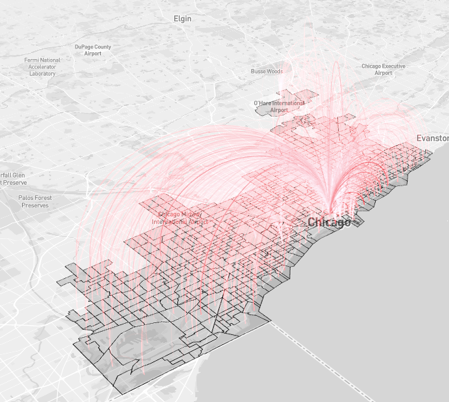
\includegraphics[width=1.0\textwidth]{arc-1}
    \caption{This map shows all the connections between where people live and work in Chicago.}
    \label{fig:arc-1}
\end{figure}

\begin{figure}[H]
    \centering
    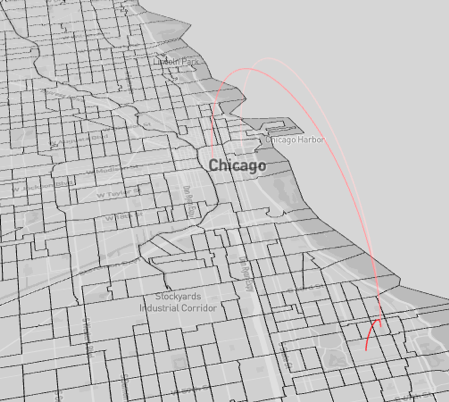
\includegraphics[width=1.0\textwidth]{arc-2}
    \caption{This map shows the connections between a people living Hyde Park who either commute to the University of Chicago or the The Loop}
    \label{fig:arc-2}
\end{figure} \\

In order to correlate the LEHD calculated centrality measures to other datasets I use the following considerations.  When comparing eigenvector centrality to home values, I calculate centrality on the neighborhood level as this is the most fine-grained data level that is available through Zillow.  When comparing centrality with data that is only available from the City of Chicago such as Business Licenses and Crime, I calculate centrality on the census block level for the entire Chicago MSA which includes many tracts outside of the City of Chicago Boundary and counties in Wisconsin and Indiana but restrict my analysis to census blocks within the City of Chicago boundary.

Real estate listing data is provided by Zillow, an online real estate database company that tracks detailed listing data of home sales throughout the US starting in 1994.  They publish data of home sales for the top 50 markets on the neighborhood level.  In my paper I use the following statistics they publish:
\begin{enumerate}
\item Median List Price Per Square Foot (\$)
\item Monthly Home Sales (Number, Seasonably Adjusted)
\item Age of Inventory (Days)
\item Median Rent List Price (\$), 1-Bedroom
\end{enumerate}
Since I am comparing real estate prices to neighborhood rankings, I make the following adjustments to be able to compare the data.  First I normalize each neighborhood to it's initial value to get an index of the statistic over time.  Next I divide by the median value for all neighborhoods in Chicago for the given time period.  The result is a statistic that shows how the neighborhood compares to other neighborhoods in Chicago over time.  If the value is less than 1, then it is below average whereas if it is greater than 1 it is above average. \\
For a complete overview of how data was collected, cleaned, visualized, and calculated, I provide the scripts and programs I used on github at \url{https://github.com/b-nroths/chi-data}. 

\section{Methods}
In order to find the employment centers of a city I will use a setup based on eigenvector centrality that has been used in studying networks such as trade routes, social networks, and webpages.  The goal of the method is to take a network of linked entities and to output the most influential nodes in the network graph.  The definition of influential varies depending on the context of how the problem is set up and what the nodes and edges represent.  For example, in a social network, the most important node is the person who is connected to the most important people or in the “center”.  In a network of cities that trade with each other, the edges might represent the distance between cities.  The edges can either represent a connection, in which case the matrix is called an adjacency matrix and is filled with 1 and 0’s depending on if two nodes are connected to each other or the matrix could represent the strength of connection between two nodes, for example in the trading routes example it could be the distance between two cities.  In this case it is common to normalize the distances to the sum of each column is equal to one. \\

Before I demonstrate how the network matrix is built in the context of this paper, it is important to understand why we are guaranteed a positive eigenvalue from the following theorem proven by Oskar Perron and Georg Forbenius.

\theoremstyle{definition}
\begin{theorem}[Perron-Frobenius Theorem]
\label{Perron-Frobenius Theorem}
Let $C$ $\in$ $\mathbb{R}^{nxn}$ represent a nonnegative primitive matrix (i.e. $C$: $C_{i,j}$ $>$ 0).  There exists a positive real number $\lambda_{max}$, such that:
\begin{enumerate}
\item $\lambda_{max}$ $>$ 0
\item $\lambda_{max}$ has a unique (up to a constant) eigenvector $v$ which has all positive entries
\item $\lambda_{max}$ $>$ $|\lambda|$ for any eigvenvalue $\lambda$ $\neq$ $\lambda_{max}$
\end{enumerate}

\end{theorem}

\begin{theorem}
A column stochastic matrix will always has an eigenvalue 1. All other eigenvalues are in absolute
value smaller or equal to 1.
\end{theorem}

\\ 

To illustrate the network I will explore in my paper, consider a simplified example of a city of 110 people, 100 of whom live Downtown and 10 of whom live in Hyde Park.  Of the 100 people who live downtown, 90 works downtown and 10 works in Hyde Park while of the 10 people, 5 work downtown and 5 work in Hyde Park.  This network can be represented by the following matrices. 

\begin{equation}
      C
   =
  \begin{bmatrix}
    hyde park->hyde park  & hyde park->downtown\\
    downtown->hyde park  & downtown->downtown
  \end{bmatrix} = 
  \begin{bmatrix}
    5 & 10\\
    5 & 90 
  \end{bmatrix}
\end{equation}

\begin{equation}
      l
   =
  \begin{bmatrix}
    hyde park\\
    downtown
    
  \end{bmatrix} = 
  \begin{bmatrix}
    10\\
    100 
  \end{bmatrix}
\end{equation}

\begin{equation}
      w
   =
  \begin{bmatrix}
    hyde park\\
    downtown
  \end{bmatrix} = 
  \begin{bmatrix}
    15\\
    95
  \end{bmatrix}
\end{equation}

From this information we can create a commuting matrix which normalizes the flow between regions of the city and transforms the “live” matrix (2) into the “work” matrix (3).  This transforms the above matrices into the following equation.

\begin{equation}C w = l\end{equation}
\begin{equation} 
  \begin{bmatrix}
    5/15 & 5/95\\
    10/15 & 90/95
  \end{bmatrix}
  \begin{bmatrix}
    15\\
    95
  \end{bmatrix}
  = 
  \begin{bmatrix}
    10\\
    100
  \end{bmatrix}
\end{equation}

We can also calculate write out the commuting flow from work to home as

\begin{center}C $l$ = $w$\end{center}
\begin{equation} 
  \begin{bmatrix}
    0.5 & 0.1\\
    0.5 & 0.9
  \end{bmatrix}
  \begin{bmatrix}
    10\\
    100
  \end{bmatrix}
  = 
  \begin{bmatrix}
    15\\
    95
  \end{bmatrix}
\end{equation}

Lastly, I will create a network from the dataset which represents a theoretical economy within the city.  Instead of people, I consider the flow of money between regions modeled by the salary of workers that commute between regions.  The first model will be the total flow of money between regions represented by the sum of the salaries of all the workers who commute between regions.  For example, if 10 people commute from Hyde Park to Downtown and they each make an average of \$2,500 per month I will consider the money flow between Hyde Park and downtown to be \$25,000.  In my dataset, salaries are broken down into three ranges less than \$1,250, \$1,250-\$3,333 and over \$3,333.  To simplify the problem, I will represent the buckets as \$1,250, \$2,500, and \$5,000.  Consider the same commuting flows as above but now with income added according to the following breakout.\\

\begin{adjustbox}{center}
 \begin{tabular}{||c | c c c | c | c | c||} 
 \hline
 & \$1,250 & \$2,500 & \$5,000 & Total People & Total Salaries\\[0.5ex] 
 \hline\hline
 $Hyde Park -> Hyde Park$ & 1 & 2 & 2 & 5 & \$16,250 \\ 
 $Hyde Park -> Downtown$ & 2 & 3 & 5 & 10 & \$35,000 \\
 $Downtown -> Hyde Park$ & 0 & 1 & 4 & 5 & \$22,500 \\ 
 $Downtown -> Downtown$ & 10 & 20 & 60 & 90 & \$362,500 \\ 
 \hline
 \end{tabular}
\end{adjustbox}\\ \\

This is represented by the following matrix.\\

\begin{equation}
  C =
  \begin{bmatrix}
   Salaries_{HP->HP}  & Salaries_{HP->D}\\
   Salaries_{D->HP}  & Salaries_{D->D}
    
  \end{bmatrix} = 
  \begin{bmatrix}
    \$16,250 & \$35,000\\
    \$22,500 & \$362,500 
  \end{bmatrix} = 
  \begin{bmatrix}
    .419 & .088\\
    .580 & .912
  \end{bmatrix}
\end{equation}
\\
Next, I take the $C$ matrix in (5), (6), \& (7) and computing the corresponding eigenvectors and eigenvalues.\\

\begin{center}
Eigenvalue and Eigenvector for (5) \\
\begin{tabular}{||c | c c ||} 
 \hline
 & $\lambda_1$ = 1.0 & $\lambda_2$ = 0.28\\[0.5ex] 
 \hline\hline
 $Downtown$ & 0.99689815 & 0.70710678\\
 $Hyde Park$ & 0.07870249 & -0.70710678  \\ 
 \hline
 \end{tabular} \\ 
 
Eigenvalue and Eigenvector for (6) \\
\begin{tabular}{||c | c c ||} 
 \hline
 & $\lambda_1$ = 1.0 & $\lambda_2$ = 0.4\\[0.5ex] 
 \hline\hline
 $Downtown$ & 0.98058068 & 0.70710678 \\
 $Hyde Park$ & 0.19611614 & -0.70710678  \\ 
 \hline
 \end{tabular} \\ 
 
Eigenvalue and Eigenvector for (7) \\
\begin{tabular}{||c | c c ||} 
 \hline
 & $\lambda_1$ = 1.0 & $\lambda_2$ = 0.33\\[0.5ex] 
 \hline\hline
 $Downtown$ & 0.98869689 & 0.70710678 \\
 $Hyde Park$ & 0.14992818 & -0.70710678  \\ 
 \hline
 \end{tabular}
 \end{center}

These results will demonstrate a few things.  First, note that the principle eigenvalue is 1.0 as expected from the theorem above.  The vector that corresponds to the principle eigenvalue is the Gould Index of Accessibility in the network and represents the relative strength of each node in the principle network.  In the three examples above you can see that the Downtown area dominates this vector.  The second eigenvalue represents a "pull out" of the principle network.  It is important to remember that the second eigenvector will be orthogonal to the principle eigenvector and represents a completely different sub-network.  In the system in equation 5 and 7 the second eigenvalue is lower which indicates the dominance of the first eigenvalue compared to the network examined in the 6 equation.  These results have a similar interpretation to the previous example where the principle eigenvector show the most dominant network of living regions.  The eigenvector that corresponds to the principle eigenvalue are the relative ranking of regions in this setting.  \\

Also, consider a more balanced commuting flow with it's corresponding eigenvalues.

\begin{center}C $l$ = $w$\end{center}
\begin{equation} 
  \begin{bmatrix}
    0.60 & 0.55\\
    0.40 & 0.45
  \end{bmatrix}
  \begin{bmatrix}
    50\\
    50
  \end{bmatrix}
  = 
  \begin{bmatrix}
    57.5\\
    42.5
  \end{bmatrix}
\end{equation}

\begin{center} 
Eigenvalue and Eigenvector for (8) \\
\begin{tabular}{||c | c c ||} 
 \hline
 & $\lambda_1$ = 1.0 & $\lambda_2$ = 0.05\\[0.5ex] 
 \hline\hline
 $Downtown$ & 0.8087 & 0.70710678 \\
 $Hyde Park$ & 0.5882 & -0.70710678  \\ 
 \hline
 \end{tabular}
 \end{center}

Here not only is the primary eigenvector more equal across neighborhoods with values of $0.8087$ and $0.5882$, the value of the second eigenvalue is also very small compared to the first $\lambda_2$ = 0.05.  This means that the majority of the network is explained by it's primary eigenvalue. \\
 Next I will use this same set up to analyze the neighborhoods of Chicago using the LEHD dataset.

\section{Results}
\subsection{Centrality for Employment}
First, I will study what neighborhoods are the most important for different job sectors, income ranges, and age profiles.  I will use the commuting matrix described in equation 6 to rank the neighborhoods according to the eigenvector that corresponds to the principle eigenvalue.  Answering the question \textit{How important is a neighborhood to jobs in a specific industry, age group or salary range?}  To do this, I create a connectivity matrix over all neighborhoods in the Chicago MSA and rank them from the years 2002 - 2015.  Below I list the top 10 neighborhoods ranked according to the eigenvalue that corresponds to the principle eigenvector.  In the last column I note the percentage change from 2002 to 2015 of the neighborhood. \\

\begin{adjustbox}{center}
\begin{tabular}{||c | c c c c c c c c c c c c c c | c||} 
 \hline
 & 2002 & 2003 & 2004 & 2005 & 2006 & 2007 & 2008 & 2009 & 2010 & 2011 & 2012 & 2013 & 2014 & 2015 & \%\\[0.5ex] 
 \hline\hline
The Loop       & 0.958 & 0.952 & 0.954 & 0.939 & 0.947 & 0.955 & 0.947 & 0.960 & 0.961 & 0.962 & 0.962 & 0.964 & 0.962 & 0.964 & +0.60\% \\
Streeterville  & 0.162 & 0.176 & 0.180 & 0.203 & 0.206 & 0.168 & 0.174 & 0.157 & 0.146 & 0.144 & 0.134 & 0.131 & 0.115 & 0.129 & -20.4\% \\
O'Hare Airport & 0.121 & 0.084 & 0.079 & 0.078 & 0.057 & 0.079 & 0.120 & 0.063 & 0.077 & 0.070 & 0.090 & 0.074 & 0.095 & 0.082 & -32.3\% \\
South Loop     & 0.102 & 0.124 & 0.113 & 0.125 & 0.115 & 0.110 & 0.114 & 0.109 & 0.075 & 0.081 & 0.086 & 0.089 & 0.090 & 0.065 & -37.0\% \\
River North    & 0.074 & 0.070 & 0.076 & 0.084 & 0.083 & 0.082 & 0.085 & 0.079 & 0.097 & 0.091 & 0.098 & 0.094 & 0.099 & 0.116 & +56.8\% \\
Bronzeville    & 0.041 & 0.036 & 0.049 & 0.056 & 0.016 & 0.044 & 0.050 & 0.048 & 0.037 & 0.034 & 0.011 & 0.014 & 0.013 & 0.011 & -73.2\% \\
Near North     & 0.074 & 0.098 & 0.085 & 0.101 & 0.098 & 0.091 & 0.088 & 0.088 & 0.085 & 0.086 & 0.073 & 0.070 & 0.073 & 0.074 & +0.00\% \\
West Loop Gate & 0.073 & 0.084 & 0.083 & 0.097 & 0.085 & 0.087 & 0.087 & 0.085 & 0.083 & 0.094 & 0.089 & 0.094 & 0.099 & 0.105 & +43.8\% \\
West Town      & 0.039 & 0.052 & 0.049 & 0.052 & 0.054 & 0.048 & 0.049 & 0.049 & 0.041 & 0.045 & 0.046 & 0.042 & 0.047 & 0.053 & +35.9\% \\
Archer Heights & 0.034 & 0.039 & 0.032 & 0.033 & 0.034 & 0.027 & 0.031 & 0.025 & 0.028 & 0.019 & 0.014 & 0.013 & 0.022 & 0.019 & -44.2\% \\
Hyde Park      & 0.049 & 0.043 & 0.063 & 0.092 & 0.077 & 0.080 & 0.100 & 0.067 & 0.096 & 0.087 & 0.094 & 0.088 & 0.088 & 0.089 & +81.6\% \\
 \hline
 \end{tabular}
\end{adjustbox}
\\

\begin{figure}[H]
    \centering
    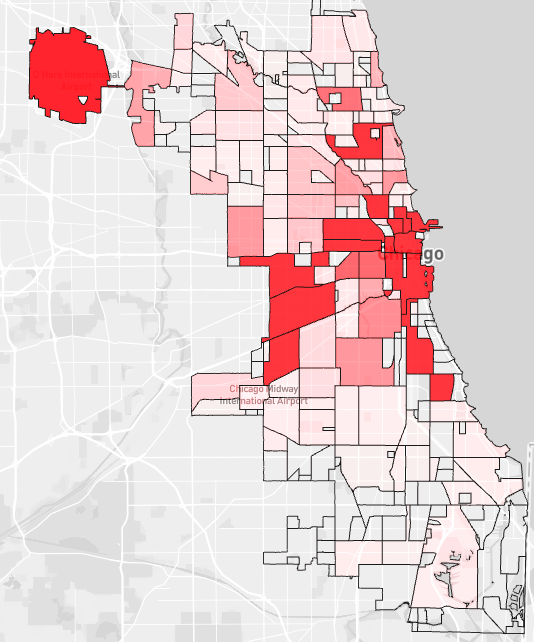
\includegraphics[width=0.31\textwidth]{Jobs-S000-2002}
    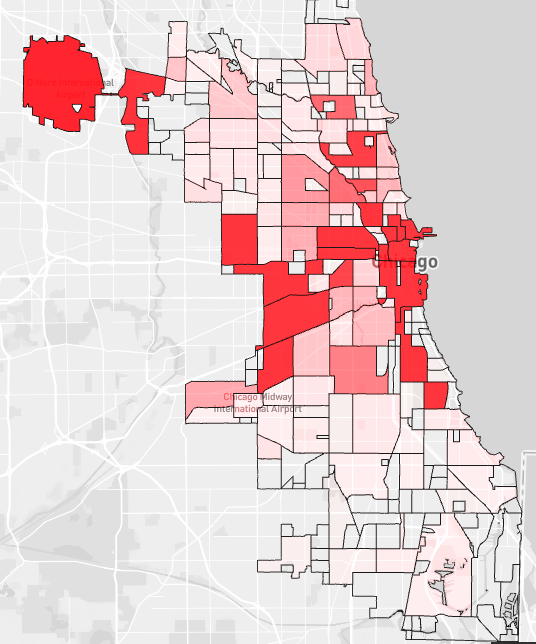
\includegraphics[width=0.31\textwidth]{Jobs-S000-2008}
    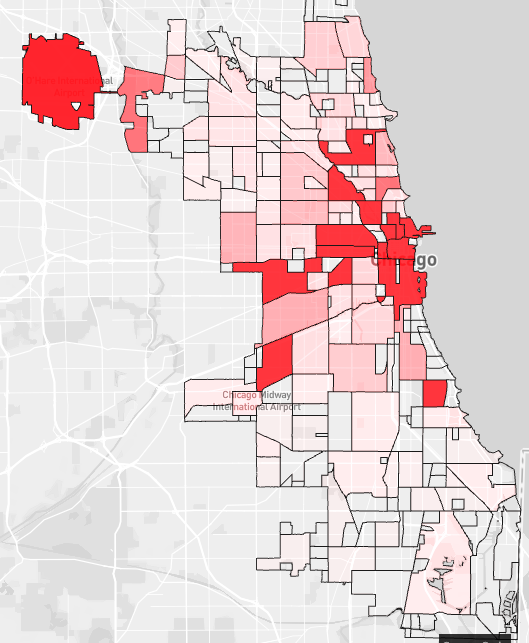
\includegraphics[width=0.31\textwidth]{Jobs-S000-2015}

        
    \caption{This map shows the eigenvector corresponding to the principle eigenvalue for 2002, 2008, and 2015}
    \label{fig:Jobs-S000-2008}
\end{figure}

As can be seen in the map and table employment is Chicago is highly concentrated in the downtown The Loop neighborhood which consistently is ranked above .95 and dominating the rank of all other neighborhoods.  Other consistently important neighborhoods include include Streeterville which is just north of The Loop as well as O'Hare Airport. Looking at the change in rankings overtime can give us an interesting view of how neighborhoods are becoming more or less important centers of employment over time.  For example, West Loop gate which is the neighborhood just west of the Chicago River has become much more important relative to other neighborhoods.  There have been a number of high tech companies that have opened offices in the West Loop since 2014 such Uber and Google to name a few.\footnote{https://www.builtinchicago.org/2014/09/18/meet-neighbors-4-tech-companies-sign-huge-leases-west-loop}.  Hyde Park has also grown in importance driven by the census blocks that cover the University and Harper Court.\footnote{https://fiftythird.uchicago.edu/category/tags/harper-court-partners} \footnote{this feels anecdotal, bring in the other LEHD employment data, how is this conclusion different from just analyzing the counts?}\\

Another interesting view of the data is to look at the value and location of the second eigenvector of the network over time.  As explained before the second eigenvector will depict a completely orthogonal network compared to the primary eigenvector and can give an idea of how more or less important the primary network is than the next network. One way to think of the second eigenvector would be a completely different "economy" that is somehow separate from the primary "economy" in the city, for example it is common for people to live between these regions with less access to the primary region.  In the graph below I show the value of the second eigenvalue over time which decreases from 0.51 to 0.41 from 2002 to 2015.  This means that compared to the primary network the influence of the secondary network is decreasing.  There could be a few reasons for this, for example the primary network could be increasing in size from outside forces or perhaps people from the secondary network are joining the primary network.  An alternative explanation is that people are leaving the secondary network. TODO: any way to show this?\\
\begin{center}
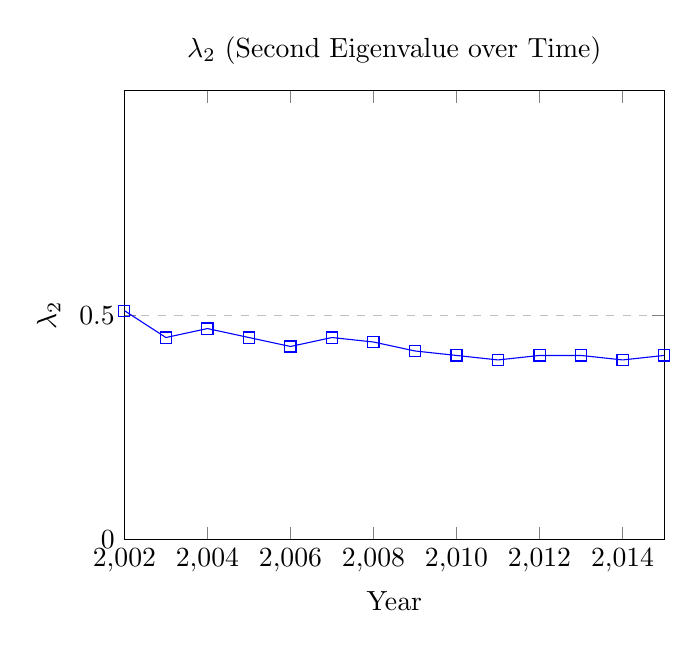
\begin{tikzpicture}
\begin{axis}[
    title={$\lambda_2$ (Second Eigenvalue over Time)},
    xlabel={Year},
    ylabel={$\lambda_2$},
    xmin=2002, xmax=2015,
    ymin=0, ymax=1,
    xtick={2002, 2004, 2006, 2008, 2010, 2012, 2014},
    ytick={0, 0.5},
    legend pos=north west,
    ymajorgrids=true,
    grid style=dashed,
]
 
\addplot[
    color=blue,
    mark=square,
    ]
    coordinates {
    (2002, 0.51)
    (2003, 0.45)
    (2004, 0.47)
    (2005, 0.45)
    (2006, 0.43)
    (2007, 0.45)
    (2008, 0.44)
    (2009, 0.42)
    (2010, 0.41)
    (2011, 0.40)
    (2012, 0.41)
    (2013, 0.41)
    (2014, 0.40)
    (2015, 0.41)
    };

\end{axis}
\end{tikzpicture}
\end{center}

Next I will take a look at how the different neighborhoods specialize in different jobs.  Below I map the primary eigenvalue for all job categories, ages, and income levels in three years, 2002, 2008, and 2015.

\begin{figure}[H]
    \centering
    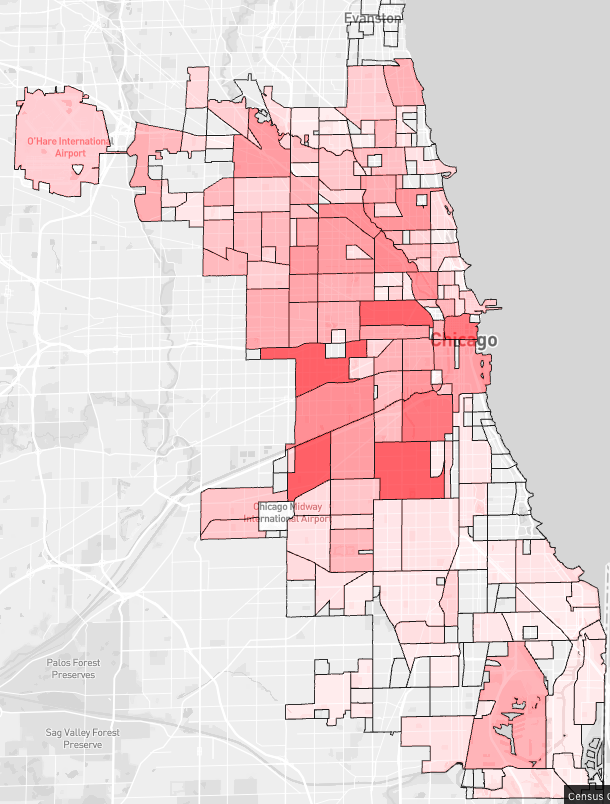
\includegraphics[width=0.31\textwidth]{Jobs-SI001-2015}
    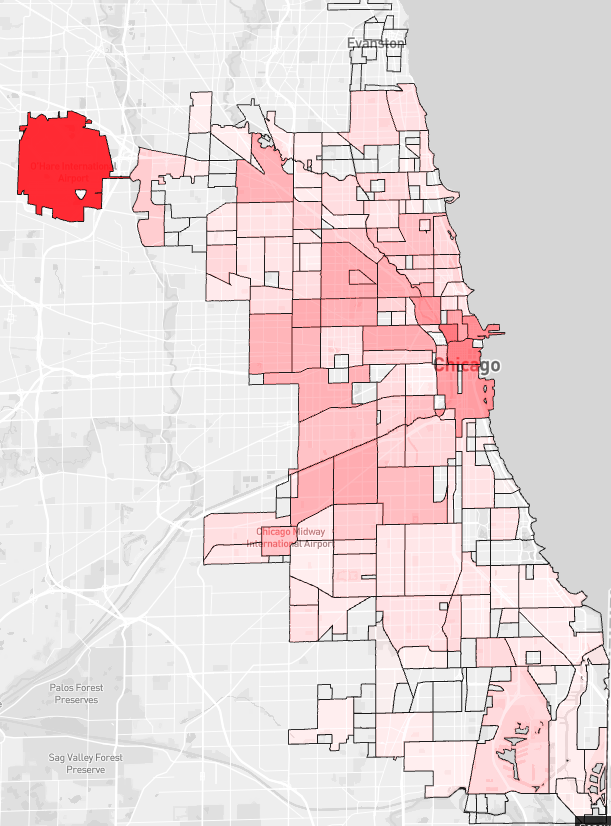
\includegraphics[width=0.31\textwidth]{Jobs-SI002-2015}
    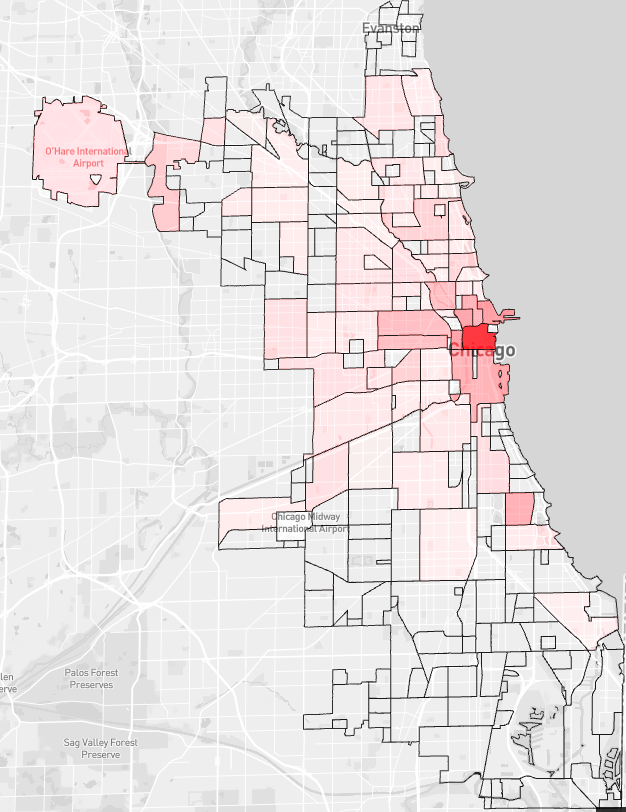
\includegraphics[width=0.31\textwidth]{Jobs-SI003-2015}
    \caption{These maps show the eigenvectors for the three different industry categories: Goods Producing (left), Trade, Transportation, Utilities (center), Other (right) for 2015}
    \label{fig:Jobs-S000-2008}
\end{figure}

This method of centrality importance is clearly able to pull out the different networks of employment in Chicago such as how dispersed the Goods Producing sector is compared to the Trade, Transportation, and Utilities sector which is dominated by O'Hare International Airport.  The Other category is dominated by The Loop area where most of the jobs in the city are located. \\

Lastly I will look at the centrality importance of jobs at different income levels.

\begin{figure}[H]
    \centering
    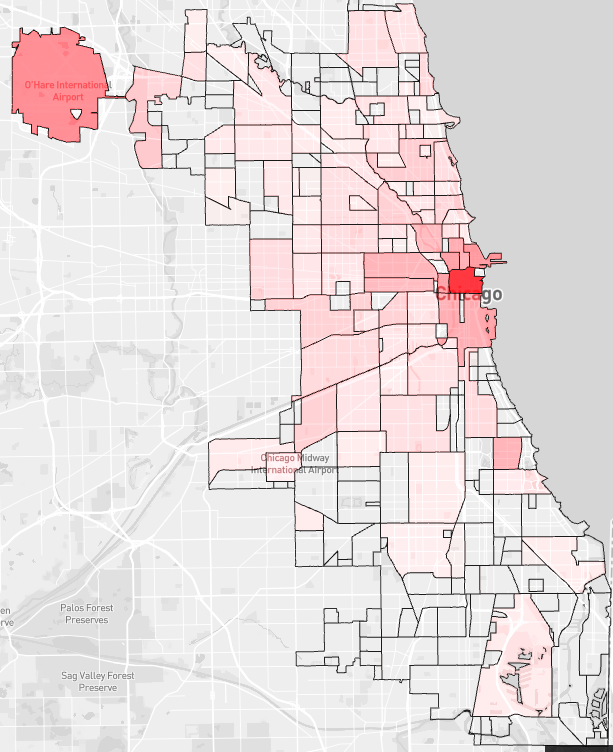
\includegraphics[width=0.31\textwidth]{Jobs-SE001-2015}
    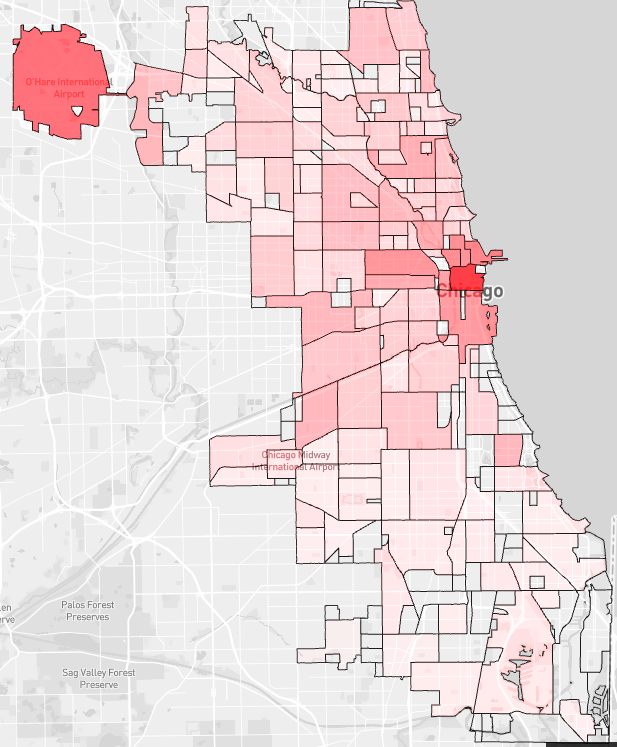
\includegraphics[width=0.31\textwidth]{Jobs-SE002-2015}
    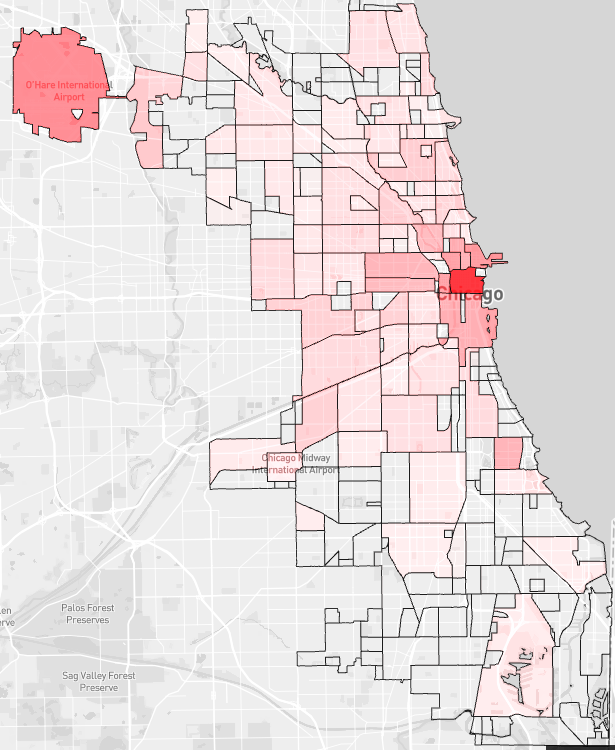
\includegraphics[width=0.31\textwidth]{Jobs-SE003-2015}
    \caption{These maps show the eigenvectors for the three different salary levels: Under \$1,250 left, \$1,250 - \$3,333 center, Over \$3,333 right for 2015.}
    \label{fig:Jobs-S000-2008}
\end{figure}

Above I used the theory of eigenvector centrality to rank the most important neighborhoods of employment for neighborhoods in Chicago.  This perspective gives us a rich view of the composition of a neighborhood as well as how it changes over time in comparision to other neighborhoods in the city.

\subsection{Centrality for Housing}
Similar to how we calculated centrality for employment we can use the same setup to calculate the centrality for housing, answering the question \textit{What neighborhoods are the most important for housing?}.  We can also break down the neighborhoods by most important for High/Middle/and Low income earners based off of the LEHD Dataset.  The top neighborhoods 10 neighborhoods based on their centrality from 2002 are listed below. \\

\begin{table}[h]\centering
\caption{Top Neighborhoods}\label{thelabel}

\begin{adjustbox}{center}
\begin{tabular}{||c | c c c c c c c c c c c c c | c ||} 
 \hline
 & 2002 & 2003 & 2005 & 2006 & 2007 & 2008 & 2009 & 2010 & 2011 & 2012 & 2013 & 2014 & 2015 & | \%\\[0.5ex] 
 \hline\hline
Logan Square     & 0.303 & 0.307 & 0.296 & 0.287 & 0.207 & 0.296 & 0.201 & 0.313 & 0.316 & 0.323 & 0.333 & 0.340 & 0.322 & 6.271\% \\
West Rogers Park & 0.220 & 0.221 & 0.224 & 0.230 & 0.201 & 0.221 & 0.209 & 0.246 & 0.260 & 0.261 & 0.254 & 0.245 & 0.239 & 8.636\% \\
Gresham          & 0.238 & 0.239 & 0.233 & 0.231 & 0.245 & 0.242 & 0.254 & 0.202 & 0.205 & 0.213 & 0.193 & 0.201 & 0.215 & -9.664\% \\
Portage Park     & 0.188 & 0.185 & 0.181 & 0.182 & 0.214 & 0.191 & 0.220 & 0.201 & 0.203 & 0.190 & 0.198 & 0.188 & 0.189 & 0.532\% \\
Archer Heights   & 0.181 & 0.178 & 0.186 & 0.182 & 0.187 & 0.173 & 0.185 & 0.198 & 0.173 & 0.175 & 0.184 & 0.186 & 0.188 & 3.867\% \\
Little Village   & 0.208 & 0.200 & 0.196 & 0.193 & 0.201 & 0.176 & 0.201 & 0.178 & 0.171 & 0.183 & 0.187 & 0.197 & 0.188 & -9.615\% \\
Albany Park      & 0.189 & 0.195 & 0.179 & 0.172 & 0.144 & 0.181 & 0.133 & 0.186 & 0.198 & 0.201 & 0.193 & 0.183 & 0.179 & -5.291\% \\
Englewood        & 0.247 & 0.244 & 0.236 & 0.239 & 0.258 & 0.223 & 0.252 & 0.197 & 0.185 & 0.178 & 0.172 & 0.177 & 0.179 & -27.530\% \\
Bridgeport       & 0.139 & 0.147 & 0.146 & 0.157 & 0.171 & 0.165 & 0.181 & 0.189 & 0.171 & 0.176 & 0.175 & 0.171 & 0.174 & 25.180\% \\
Rogers Park      & 0.154 & 0.151 & 0.150 & 0.159 & 0.133 & 0.155 & 0.127 & 0.158 & 0.172 & 0.175 & 0.177 & 0.175 & 0.174 & 12.987\% \\ \hline
 \end{tabular}
\end{adjustbox}
\end{table}
\\

Some things to notice right away are that the rankings are much more stable than they were for the employment dataset as most neighborhoods only increasing or decreasing in the single digits over the 14 year timespan.  Also, the distributions of the rankings are a lot more even across neighborhoods compared to the employment dataset which was dominated by The Loop neighborhood. \\

\begin{figure}[H]
    \centering
    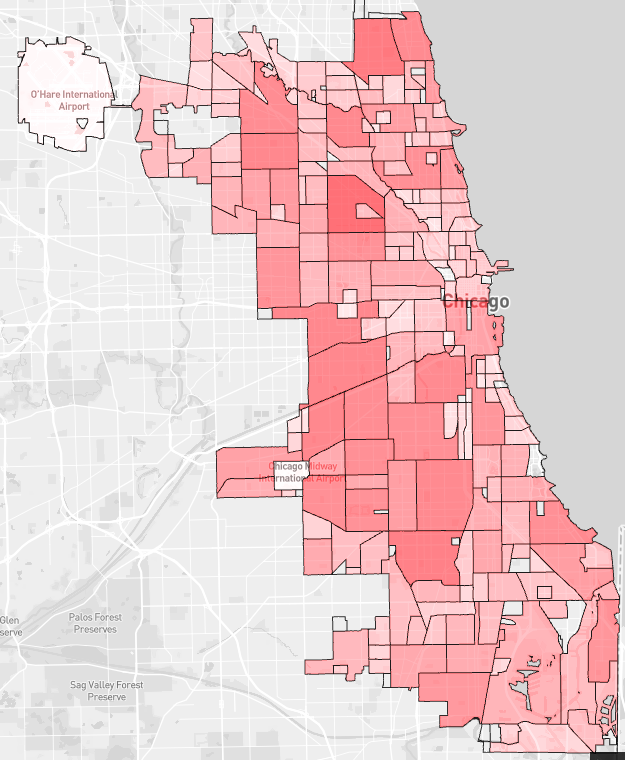
\includegraphics[width=1.0\textwidth]{Houses-S000-2015}
    \caption{This map shows the eigenvector that corresponds to the principal eigenvalue for the housing pagerank algorithm.}
    \label{fig:Houses-S000-2015}
\end{figure}

After the centrality measurements are created we can start to ask interesting questions such as how neighborhoods are changing overtime in comparison to each other.  The main dimensions I will look at are how the age and income are affecting neighborhoods in Chicago.  Below are tables of the top 10 neighborhoods by centrality ranking for Young/Old workers and Low-Income/High Income workers.\\

\begin{table}[h]\centering
\caption{Top Neighborhoods for Young Workers (Age < 29)}\label{thelabel}
\begin{adjustbox}{center}
\begin{tabular}{||c | c c c c c c c c c c c c c c | c ||} 
 \hline
 & 2002 & 2003 & 2004 & 2005 & 2006 & 2007 & 2008 & 2009 & 2010 & 2011 & 2012 & 2013 & 2014 & 2015 & | \%\\[0.5ex] 
 \hline\hline
Logan Square     & 0.355 & 0.364 & 0.341 & 0.353 & 0.338 & 0.262 & 0.368 & 0.235 & 0.388 & 0.385 & 0.398 & 0.408 & 0.391 & 0.385 & +8.451\% \\
Little Village   & 0.248 & 0.247 & 0.244 & 0.253 & 0.234 & 0.235 & 0.200 & 0.228 & 0.207 & 0.202 & 0.224 & 0.224 & 0.230 & 0.217 & -12.500\% \\
Gresham          & 0.194 & 0.201 & 0.215 & 0.197 & 0.190 & 0.209 & 0.219 & 0.227 & 0.164 & 0.173 & 0.174 & 0.158 & 0.187 & 0.209 & +7.732\% \\
Englewood        & 0.244 & 0.257 & 0.253 & 0.239 & 0.234 & 0.262 & 0.226 & 0.254 & 0.183 & 0.157 & 0.165 & 0.162 & 0.175 & 0.205 & -15.984\% \\
Archer Heights   & 0.197 & 0.184 & 0.191 & 0.199 & 0.191 & 0.198 & 0.174 & 0.205 & 0.209 & 0.166 & 0.186 & 0.195 & 0.198 & 0.189 & -4.061\% \\
Lake View        & 0.155 & 0.171 & 0.191 & 0.185 & 0.212 & 0.186 & 0.214 & 0.156 & 0.240 & 0.215 & 0.208 & 0.191 & 0.177 & 0.187 & +20.645\% \\
Brighton Park    & 0.187 & 0.189 & 0.182 & 0.186 & 0.189 & 0.145 & 0.158 & 0.145 & 0.156 & 0.164 & 0.159 & 0.183 & 0.170 & 0.179 & -4.278\% \\
West Rogers Park & 0.169 & 0.165 & 0.168 & 0.176 & 0.169 & 0.169 & 0.178 & 0.185 & 0.192 & 0.206 & 0.208 & 0.191 & 0.175 & 0.178 & +5.325\% \\
Rogers Park      & 0.142 & 0.139 & 0.140 & 0.144 & 0.153 & 0.126 & 0.145 & 0.135 & 0.154 & 0.166 & 0.154 & 0.154 & 0.158 & 0.174 & +22.535\% \\
Marquette Park   & 0.140 & 0.144 & 0.150 & 0.176 & 0.180 & 0.164 & 0.151 & 0.160 & 0.131 & 0.132 & 0.135 & 0.124 & 0.142 & 0.167 & +19.286\% \\
Gage Park        & 0.155 & 0.162 & 0.160 & 0.142 & 0.150 & 0.153 & 0.141 & 0.144 & 0.155 & 0.142 & 0.137 & 0.174 & 0.166 & 0.166 & +7.097\% \\
 \hline
 \end{tabular}

\end{adjustbox}
 \end{table}
 
\begin{table}[h]\centering
\caption{Top Neighborhoods for Old Workers (Age over 55)}\label{thelabel}
\begin{adjustbox}{center}
\begin{tabular}{||c | c c c c c c c c c c c c c c | c ||} 
 \hline
 & 2002 & 2003 & 2004 & 2005 & 2006 & 2007 & 2008 & 2009 & 2010 & 2011 & 2012 & 2013 & 2014 & 2015 & | \%\\[0.5ex] 
 \hline\hline
West Rogers Park & 0.229 & 0.248 & 0.234 & 0.220 & 0.225 & 0.186 & 0.247 & 0.183 & 0.273 & 0.293 & 0.301 & 0.302 & 0.273 & 0.281 & +22.707\% \\
Logan Square     & 0.231 & 0.224 & 0.223 & 0.201 & 0.211 & 0.129 & 0.196 & 0.167 & 0.234 & 0.225 & 0.240 & 0.246 & 0.265 & 0.239 & +3.463\% \\
Portage Park     & 0.183 & 0.202 & 0.213 & 0.204 & 0.189 & 0.220 & 0.219 & 0.239 & 0.216 & 0.240 & 0.225 & 0.215 & 0.242 & 0.235 & +28.415\% \\
Gresham          & 0.314 & 0.292 & 0.319 & 0.312 & 0.301 & 0.280 & 0.261 & 0.283 & 0.238 & 0.238 & 0.221 & 0.220 & 0.228 & 0.229 & -27.070\% \\
Jefferson Park   & 0.193 & 0.200 & 0.185 & 0.194 & 0.184 & 0.189 & 0.225 & 0.194 & 0.231 & 0.208 & 0.204 & 0.214 & 0.235 & 0.208 & +7.772\% \\
Bridgeport       & 0.119 & 0.139 & 0.148 & 0.134 & 0.151 & 0.189 & 0.170 & 0.190 & 0.200 & 0.185 & 0.191 & 0.209 & 0.197 & 0.194 & +63.025\% \\
Albany Park      & 0.155 & 0.164 & 0.159 & 0.164 & 0.150 & 0.118 & 0.176 & 0.121 & 0.174 & 0.179 & 0.192 & 0.182 & 0.175 & 0.186 & +20.000\% \\
Archer Heights   & 0.159 & 0.156 & 0.155 & 0.181 & 0.173 & 0.178 & 0.168 & 0.167 & 0.194 & 0.160 & 0.163 & 0.172 & 0.158 & 0.168 & +5.660\% \\
Little Village   & 0.150 & 0.154 & 0.164 & 0.162 & 0.169 & 0.181 & 0.150 & 0.196 & 0.155 & 0.145 & 0.167 & 0.163 & 0.171 & 0.161 & +7.333\% \\
West Pullman     & 0.185 & 0.205 & 0.189 & 0.177 & 0.241 & 0.172 & 0.175 & 0.179 & 0.164 & 0.153 & 0.142 & 0.138 & 0.142 & 0.161 & -12.973\% \\
 \hline
 \end{tabular}

\end{adjustbox}
\end{table}

\begin{table}[h]\centering
\caption{Top Neighborhoods for Low Income Earners}\label{thelabel}
\begin{adjustbox}{center}
\begin{tabular}{||c | c c c c c c c c c c c c c c | c ||} 
 \hline
 & 2002 & 2003 & 2004 & 2005 & 2006 & 2007 & 2008 & 2009 & 2010 & 2011 & 2012 & 2013 & 2014 & 2015 & | \%\\[0.5ex] 
 \hline\hline
Gresham           & 0.254 & 0.259 & 0.000 & 0.256 & 0.263 & 0.247 & 0.278 & 0.287 & 0.237 & 0.234 & 0.240 & 0.220 & 0.255 & 0.280 & +10.236\% \\
Englewood         & 0.310 & 0.296 & 0.000 & 0.290 & 0.314 & 0.325 & 0.292 & 0.299 & 0.245 & 0.223 & 0.227 & 0.222 & 0.257 & 0.271 & -12.581\% \\
Logan Square      & 0.272 & 0.283 & 0.000 & 0.262 & 0.247 & 0.183 & 0.255 & 0.194 & 0.293 & 0.286 & 0.284 & 0.304 & 0.280 & 0.246 & -9.559\% \\
West Rogers Park  & 0.201 & 0.224 & 0.000 & 0.232 & 0.222 & 0.190 & 0.220 & 0.195 & 0.249 & 0.272 & 0.240 & 0.248 & 0.220 & 0.218 & +8.458\% \\
Archer Heights    & 0.189 & 0.204 & 0.000 & 0.195 & 0.182 & 0.191 & 0.187 & 0.181 & 0.198 & 0.190 & 0.192 & 0.207 & 0.204 & 0.211 & +11.640\% \\
Bridgeport        & 0.158 & 0.185 & 0.000 & 0.182 & 0.195 & 0.196 & 0.191 & 0.206 & 0.217 & 0.196 & 0.207 & 0.197 & 0.186 & 0.190 & +20.253\% \\
Little Village    & 0.212 & 0.208 & 0.000 & 0.199 & 0.200 & 0.201 & 0.180 & 0.184 & 0.172 & 0.164 & 0.192 & 0.206 & 0.199 & 0.183 & -13.679\% \\
West Pullman      & 0.196 & 0.180 & 0.000 & 0.153 & 0.174 & 0.142 & 0.170 & 0.171 & 0.172 & 0.137 & 0.173 & 0.151 & 0.173 & 0.177 & -9.694\% \\
South Shore       & 0.172 & 0.153 & 0.000 & 0.166 & 0.174 & 0.184 & 0.190 & 0.203 & 0.144 & 0.161 & 0.155 & 0.152 & 0.158 & 0.176 & +2.326\% \\
Back of the Yards & 0.183 & 0.172 & 0.000 & 0.185 & 0.188 & 0.164 & 0.182 & 0.164 & 0.194 & 0.171 & 0.169 & 0.171 & 0.166 & 0.172 & -6.011\% \\
 \hline
 \end{tabular}
\end{adjustbox}
\end{table}


\begin{table}[h]\centering
\caption{Top Neighborhoods for High Income Earners}\label{thelabel}
\begin{adjustbox}{center}
\begin{tabular}{||c | c c c c c c c c c c c c c c | c ||} 
 \hline
 & 2002 & 2003 & 2004 & 2005 & 2006 & 2007 & 2008 & 2009 & 2010 & 2011 & 2012 & 2013 & 2014 & 2015 & | \%\\[0.5ex] 
 \hline\hline
Logan Square     & 0.235 & 0.261 & 0.249 & 0.240 & 0.262 & 0.198 & 0.282 & 0.221 & 0.295 & 0.305 & 0.300 & 0.331 & 0.350 & 0.335 & +42.553\% \\
Lake View        & 0.331 & 0.342 & 0.307 & 0.332 & 0.331 & 0.263 & 0.319 & 0.289 & 0.345 & 0.323 & 0.359 & 0.330 & 0.312 & 0.321 & -3.021\% \\
West Rogers Park & 0.291 & 0.273 & 0.293 & 0.272 & 0.290 & 0.262 & 0.268 & 0.302 & 0.284 & 0.281 & 0.270 & 0.265 & 0.266 & 0.264 & -9.278\% \\
Lake View East   & 0.241 & 0.257 & 0.243 & 0.278 & 0.279 & 0.202 & 0.262 & 0.185 & 0.233 & 0.239 & 0.241 & 0.237 & 0.242 & 0.243 & +0.830\% \\
Jefferson Park   & 0.248 & 0.257 & 0.267 & 0.246 & 0.235 & 0.251 & 0.259 & 0.237 & 0.207 & 0.214 & 0.228 & 0.237 & 0.247 & 0.226 & -8.871\% \\
Portage Park     & 0.239 & 0.216 & 0.203 & 0.196 & 0.195 & 0.226 & 0.194 & 0.212 & 0.186 & 0.190 & 0.189 & 0.191 & 0.183 & 0.202 & -15.481\% \\
Albany Park      & 0.159 & 0.161 & 0.166 & 0.171 & 0.164 & 0.159 & 0.186 & 0.138 & 0.178 & 0.204 & 0.205 & 0.204 & 0.190 & 0.191 & +20.126\% \\
Rogers Park      & 0.166 & 0.174 & 0.167 & 0.180 & 0.186 & 0.165 & 0.181 & 0.157 & 0.191 & 0.190 & 0.191 & 0.188 & 0.175 & 0.187 & +12.651\% \\
Ravenswood       & 0.169 & 0.171 & 0.164 & 0.157 & 0.166 & 0.145 & 0.175 & 0.150 & 0.187 & 0.190 & 0.174 & 0.170 & 0.172 & 0.187 & +10.651\% \\
South Loop       & 0.107 & 0.104 & 0.117 & 0.159 & 0.168 & 0.191 & 0.123 & 0.180 & 0.158 & 0.173 & 0.169 & 0.175 & 0.166 & 0.178 & +66.355\% \\
 \hline
 \end{tabular}
\end{adjustbox}
\end{table}

Above we can notice a few interesting facts, for example, some neighborhoods becoming a lot more influential for young workers such as Lake View, Rogers Park, and Marquette Park while others becoming more influential for older workers such as West Rogers Park, Portage Park, Bridgeport, and Albany Park. \\

There has also have been some larger shifts in where low income workers are moving such as moving into Gresham and Bridgeport whereas High Income earners have been flocking to Logan Square, Albany Park, and especially the South Loop whose importance has risen 66\% since 2002.
\subsection{To Do: Centrality for Money Flow}
I am currently working on the computation for this section.  The idea is outlined in the methods section where I will calculate neighborhood importance based off of the money that flow between neighborhoods (this is based on salary * number of workers).  I will also add outside data from construction permits etc to help with this analysis.\cite{gould1967geographical}
\section{Conclusion}
In this paper I presented a novel application of eigenvector centrality to dataset of Chicago's neighborhoods.  After exploring the data through visualizations, I derived the math necessary for this application and outlined three examples where eigenvector centrality can help explore attributes of Chicago neighborhoods.  First, I looked at how jobs were distributed across the city.  In this analysis I found how employment was centralized in the Loop.  While jobs in some industries such as Goods Producing are also located a west of downtown, The Loop neighborhood ranked at .95 while the next closest neighborhood ranked .17.  Even low-income jobs were concentrated in The Loop which was surprising.  While The Loop was a mixing pot of employment across industries, incomes, and ages, Housing centrality was much more segregated and dispersed throughout the city.  For example, I found that 
\bibliographystyle{unsrt}
\bibliography{reference}



\end{document}








